\chapter{Reinforcement Learning (RL)}
\label{ch-RL}
\begin{figure}[h!]
\centering
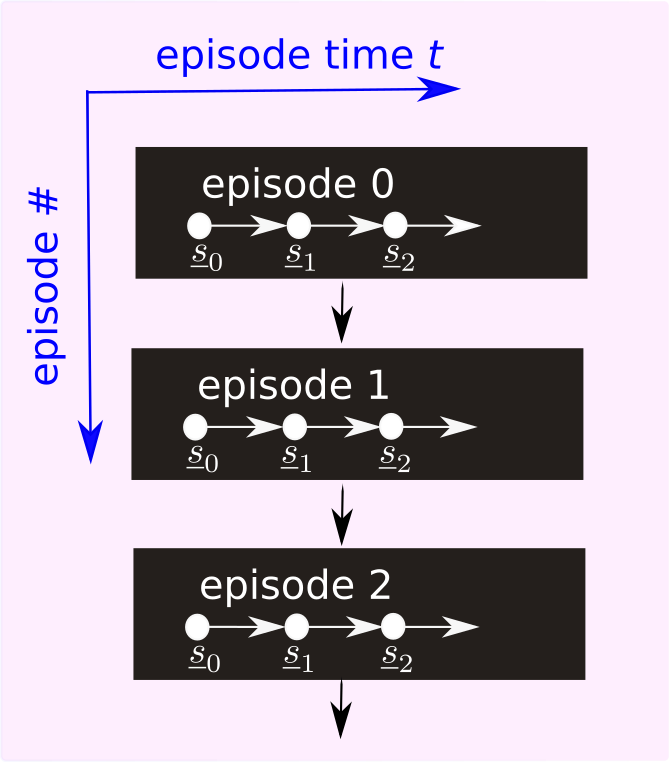
\includegraphics[width=3in]{RL/episodes.png}
\caption{Axes 
for episode time and episode number.} 
\label{fig-epi}
\end{figure}

I based this chapter on the following 
references. Refs.\cite{fox}\cite{levine}

In RL, we consider an \qt{agent} or
robot that
is learning. 

Let $T\in \ZZ_{>0}$ be the duration time
of an {\bf episode} of learning.
If $T=\infty$, we say that the episode
has an infinite time horizon.
A learning episode will 
 evolve
towards the right,
 for times $t=0,1, \ldots, T-1$. 
We will consider multiple learning episodes.
The episode number will
evolve from top to bottom.
This is illustrated in Fig.\ref{fig-epi}.

 Let $\rvs_t\in S_\rvs $ 
for $t\in \ZZ_{[0,T-1]}$ be random variables that record the {\bf state} of
the
agent at various times $t$.

Let $\rva_t\in S_\rva$ for 
$t\in \ZZ_{[0,T-1]}$ be random variables that record the {\bf action} of
the agent at various times $t$.

Let $\rvtheta_t\in S_\rvtheta$ 
for $t\in \ZZ_{[0,T-1]}$ be
random variables that record the
 {\bf policy parameters} 
at various times $t$.



For $\rvX\in \{\rvs, \rva, \rvtheta\}$, define $\rvX$ followed by a dot to be the vector 
\beq
\rvX. = 
[\rvX_0, \rvX_1, \ldots, \rvX_{T-1}]
\;.
\eeq
Also let
\beq
\rvX_{\geq t} = 
[\rvX_t, \rvX_{t+1}, \ldots, \rvX_{T-1}]
\;.
\eeq

\begin{figure}
\centering
$$\xymatrix{
\rvtheta_0\ar@/^1pc/[dd]&
\rvtheta_1\ar@/^1pc/[dd]&
\rvtheta_2\ar@/^1pc/[dd]&\\
\rvs_0\ar[r]\ar[d]\ar@/^1pc/[dd]&
\rvs_1\ar[r]\ar[d]\ar@/^1pc/[dd]&
\rvs_2\ar[d]\ar@/^1pc/[dd]\\
\rva_0\ar[ur]\ar[d]&
\rva_1\ar[ur]\ar[d]&
\rva_2\ar[d]
\\
\rvr_0&
\rvr_1&
\rvr_2
}$$
\caption{State-Action-Reward dynamical bnet}
\label{fig-basic-rl}
\end{figure}

Fig.\ref{fig-basic-rl} shows
the basic State-Action-Reward bnet
for an agent that is learning.
The TPMs, printed in blue, for the
bnet Fig.\ref{fig-basic-rl}, are
as follows.

\beq\color{blue}P(a_t|s_t, \theta_t)\text{ = given.}
\eeq
 $P(a_t|s_t, \theta_t)$ is called  a
{\bf policy with parameter $\theta_t$.} 

\beq\color{blue}P(s_{t}|s_{t-1}, a_{t-1})
\text{ = given.}\eeq
$P(s_t|s_{t-1}, a_{t-1})$ is called the
 {\bf TPM of the model}.
$P(s_t|s_{t-1}, a_{t-1})$ reduces to $P(s_0)$ when $t=0$.

\beq\color{blue}
P(r_t|s_t, a_t)=\delta(r_t, r(s_t, a_t)))
\;.\eeq
$r:S_\rvs\times S_\rva\rarrow \RR$ 
is a given
 {\bf one-time reward function}.


Note that 
\beq
P(s., a.|\theta.)=\prod_{t=0}^{T-1}
\{
P(s_t|s_{t-1}, a_{t-1})
P(a_t|s_t, \theta_t)\}
\;.
\eeq
Define the {\bf all times reward} 
$\Sigma$ by

\beq
\Sigma(s., a.) = 
\sum_{t=0}^{T-1}\gamma^t r(s_t, a_t)
\;.
\eeq
Here $0<\gamma<1$. 
$\gamma$, called the {\bf discount rate},
is included to assure 
convergence of $\Sigma$ when
$T\rarrow \infty$. 
If $r(s_t, a_t)< K$ for all $t$, then
$\Sigma< K \frac{1}{1-\gamma}$.

Define the {\bf objective (i.e., goal)
 function}
$E\Sigma(\theta.)$ by

\beq
E\Sigma(\theta.)=
E_{\rvs., \rva.|\theta.}
\Sigma(\rvs., \rva.)=
\sum_{s., a.}
P(s., a.|\theta.)\Sigma(s., a.)
\eeq
The goal of RL  is to
maximize the 
objective function over
its parameters $\theta.$.
The parameters $\theta^*.$ that 
maximize the objective function 
are the optimum strategy:

\beq 
\theta.^* = \argmax_{\theta.}
E\Sigma(\theta.)
\eeq

\hrule
Define a {\bf future reward} for
 times $\geq t$ as:
\beq
\Sigma_{\geq t}((s_{t'},
 a_{t'})_{t'\geq t}) =
 \sum_{t'=t}^{T-1}\gamma^{t'-t} r(s_{t'}, a_{t'})
\eeq

Define the following {\bf expected conditional 
future rewards} (rewards for times 
$\geq t$,
conditioned on certain quantities
having given values):

\beqa
v_t &=& v(s_t, a_t; \theta.)=E_{\rvs., \rva.|s_t,a_t, \theta.}[\Sigma_{\geq t}]\\
V_t &=& V(s_t;\theta.)=E_{\rvs., \rva.|s_t, \theta.}[\Sigma_{\geq t}]=
E_{\rva_t|s_t, \theta.}[v(s_t, \rva_t;\theta.)]
\eeqa

$v$ is usually called $Q$
in the literature. We will
refer to $Q$ as $v$
in order to follow
a convention wherein an
$\rva_t$-average changes a lower case
letter to an upper case one.  

We will sometimes
write $v(s_t, a_t)$
instead of $v(s_t, a_t;\theta.)$.

Since $E\Sigma_{\geq t}$ only depends on
$\theta_{\geq t}$, $v(s_t, a_t;\theta.)=
v(s_t, a_t;\theta_{\geq t})$, and
$V(s_t;\theta.)=
V(s_t;\theta_{\geq t})$.

Note that the objective function 
$E\Sigma$ can be expressed in terms of 
$v_0$ by averaging over its unaveraged
parameters:
\beq
E\Sigma(\theta.)=
E_{\rvs_0,\rva_0|\theta_0}
v(\rvs_0, \rva_0;\theta.)
\eeq

Define
a {\bf one-time reward}
 and an 
{\bf expected conditional one-time  reward} as:
\beqa
r_t &=& r(s_t, a_t)\\
R_t &=& R(s_t;\theta_t)=
E_{\rva_t|s_t, \theta_t}[r(s_t, \rva_t)]\
\;.
\eeqa


\hrule

Note that

\beqa
\Sigma_{\geq t} &=& r_t + \gamma r_{t+1} 
+ \gamma^2 r_{t+2} +\ldots
+ \gamma^{T-1-t} r_{t+(T-1-t)}\\
&=& r_t + \gamma \Sigma_{\geq t+1}
\label{eq-Sigma}
;.
\eeqa

 
If we take
 $E_{\rvs., \rva.|s_t, a_t, \theta.}
[\cdot]$
of both sides of Eq.(\ref{eq-Sigma}), 
we get

\beq
v_t = r_t + \gamma E_{\rvs_{t+1},
 \rva_{t+1}|\theta.} [v_{t+1}]
\;.
\eeq
If we take $E_{\rvs., \rva.|s_t, \theta.}[\cdot]$
of both sides of Eq.(\ref{eq-Sigma}), 
we get

\beq
V_t = R_t + \gamma E_{\rvs_{t+1}|\theta.}
[V_{t+1}]
\;.
\eeq

Note that
\beqa
\Delta r_t&=& r_t -R_t\\
&=& r_t -(V_t - 
\gamma E_{\rvs_{t+1}|\theta.} [V_{t+1}])\\
&=& r_t
+ \gamma E_{\rvs_{t+1}|\theta.} [V_{t+1}]
-V_t
\;.
\eeqa
Define
\beq
\Delta v_t = v_t - V_t
\;. 
\eeq
Note that 
\beq
\Delta v_t = \Delta r_t
\;.
\eeq

Next, we will discuss 3 RL bnets
\begin{itemize}
\item
exact RL bnet 
(exact, assumes policy is known)
\item
Actor-Critic RL bnet (approximate, 
assumes
policy is known)
\item
Q function learning RL bnet (approximate, 
assumes
policy is NOT known)
\end{itemize}



\section{Exact RL bnet}

\begin{figure}
\centering
$$\xymatrix{
\rvtheta.\ar[d]\ar[dr]\ar[drr]\ar[drrr]
\ar@/_2pc/[dddddd]\\
\rvtheta_0\ar@/^1pc/[dd]&
\rvtheta_1\ar@/^1pc/[dd]&
\rvtheta_2\ar@/^1pc/[dd]&
\rvtheta_3&\\
\rvs_0\ar[r]\ar[d]\ar@/^1pc/[dd]&
\rvs_1\ar[r]\ar[d]\ar@/^1pc/[dd]&
\rvs_2\ar[r]\ar[d]\ar@/^1pc/[dd]&
\rvs_3\\
\rva_0\ar[d]\ar[ur]&
\rva_1\ar[d]\ar[ur]&
\rva_2\ar[d]\ar[ur]&
\rva_3\\
\rvr_0\ar[d]&
\rvr_1\ar[d]&
\rvr_2\ar[d]&
\rvr_3\\
\rvv_0(\cdot)\ar[d]&
\rvv_1(\cdot)\ar[l]&
\rvv_2(\cdot)\ar[l]&
\rvv_3(\cdot)\ar[l]\\
\rvtheta'.
}$$
\caption{Exact RL bnet. 
$v_t(\cdot)$ means the  array
$[v_t(s_t,a_t)]_{\forall s_t, a_t}$ 
The
following arrows 
are implicit:
 for all $t$, arrow
from $\rvtheta.\rarrow \rvv_t(\cdot)$.
We did not draw those arrows
so as not to clutter the diagram.}
\label{fig-exact-rl}
\end{figure}
An exact RL bnet is given by
 Fig.\ref{fig-exact-rl}.


Fig.\ref{fig-exact-rl} is the 
same as Fig.\ref{fig-basic-rl} but
 with more nodes added in order to
optimize the policy parameters.
The TPMs, printed
in blue, 
for the nodes not already discussed
in connection to bnet
Fig.\ref{fig-basic-rl},
are as follows.

 

\beq \color{blue}
P(\theta_t|\theta.) =
\delta(\theta_t, (\theta.)_t)
\eeq


\beq\color{blue}\forall (s_t, a_t):\;\;
P(v_t(s_t, a_t)|r_t, v_{t+1}(\cdot),\theta.)
=\delta(v_t(s_t,a_t), r_t + 
\gamma E_{\rvs_{t+1},\rva_{t+1}
|\theta.}[ v_{t+1}])
\eeq

\beq \color{blue}
P(\theta.'|\theta., v_0(\cdot))=
\delta(\theta'.,
\theta. + \alpha\partial_{\theta.}
\underbrace{E_{\rvs_0, \rva_0|\theta_0}
v(\rvs_0, \rva_0
;\theta.)}_{E\Sigma(\theta.)})
\eeq
$\alpha>0$ is called the
{\bf learning rate}. This method
of improving $\theta.$ is 
called gradient ascent.

Concerning the
gradient of the
objective function, note that

\beqa
\partial_{\theta_t}E\Sigma(\theta.)&=&
\sum_{s., a.}
\partial_{\theta_t}P(s., a.|\theta.)
\Sigma(s., a.)\\
&=& 
\sum_{s., a.}P(s., a.|\theta.)
\partial_{\theta_t}
\ln P(s., a.|\theta.)\Sigma(s., a.)
\\
&=&
E_{\rvs., \rva.|\theta.}\left\{
\partial_{\theta_t}
\ln P(a_t|s_t, \theta_t)
\Sigma(s., a.)
\right\}
\;.
\eeqa
If we run the
agent $nsam(\vecs_t)$
times and obtain
samples $s_t[i], a_t[i]$ for all $t$ and
for $i=0, 1, \ldots,nsam(\vecs_t)-1$, 
we can express this  gradient as
follows:

\beq
\partial_{\theta_t}E\Sigma(\theta.)
\approx
\frac{1}{nsam(\vecs_t)}
\sum_{i}\sum_{t=0}^{T-1}
\partial_{\theta_t}
\ln P(a_t[i]\cond s_t[i], \theta_t)
r(s_t[i], a_t[i])
\;.
\label{eq-grad-samples}
\eeq

The exact RL bnet 
Fig.\ref{fig-exact-rl} is difficult to
use to calculate the
optimum parameters $\theta^*.$.
The problem 
is that $\rvs_t$
propagates towards the future
and the $\rvv_t(\cdot)$
propagates towards the past,
so we don't have a Markov Chain 
with a chain link for each $t$ (i.e., 
a
dynamical bnet) in the 
episode time direction.
Hence,
people have come up
with approximate RL bnets
that are
doubly dynamical (i.e.,
dynamical along
the episode time and
episode number axes.)
We discuss some of those
approximate RL bnets next. 



\section{Actor-Critic RL bnet}

For the actor-critic RL 
bnet, 
we approximate Eq.(\ref{eq-grad-samples})
by

\beq
\partial_{\theta_t}E\Sigma(\theta.)
\approx
\frac{1}{nsam(\vecs)}
\sum_{i}\sum_{t=0}^{T-1}
\underbrace{
\partial_{\theta_t}
\ln P(a_t[i]\cond s_t[i], \theta_t)
}_{Actor}
\underbrace{
\Delta r_t(s_t[i], a_t[i])
}_{Critic}
\eeq


\begin{figure}
\centering
$$\xymatrix{
\rvtheta_0\ar@/^1pc/[dd]\ar@/_1pc/[ddddd]&
\rvtheta_1\ar@/^1pc/[dd]\ar@/_1pc/[ddddd]&
\rvtheta_2\ar@/^1pc/[dd]\ar@/_1pc/[ddddd]&
\rvtheta_3\\
\vec{\rvs}_0\ar[r]\ar[d]\ar@/^1pc/[dd]
\ar@/^2pc/[ddd]&
\vec{\rvs}_1\ar[r]\ar[d]\ar@/^1pc/[dd]
\ar@/^2pc/[ddd]\ar[dddl]&
\vec{\rvs}_2\ar[r]\ar[d]\ar@/^1pc/[dd]
\ar@/^2pc/[ddd]\ar[dddl]&
\vec{\rvs}_3\ar[dddl]\\
\vec{\rva}_0\ar[d]\ar[ur]\ar@/^1pc/[dd]&
\vec{\rva}_1\ar[d]\ar[ur]\ar@/^1pc/[dd]&
\vec{\rva}_2\ar[d]\ar[ur]\ar@/^1pc/[dd]&
\vec{\rva}_3\\
\vec{\rvr}_0&
\vec{\rvr}_1&
\vec{\rvr}_2&
\vec{\rvr}_3\\
\ul{\Delta \vec{v}}_0\ar[d]&
\ul{\Delta \vec{v}}_1\ar[d]&
\ul{\Delta \vec{v}}_2\ar[d]&
\ul{\Delta \vec{v}}_3\\
\rvtheta'_0&
\rvtheta'_1&
\rvtheta'_2&
\rvtheta'_3
}$$
\caption{Actor-Critic RL bnet.  }
\label{fig-ac-rl}
\end{figure}
The actor-critic RL bnet
is given by Fig.\ref{fig-ac-rl}. This
bnet is approximate and assumes
that the policy is known. The
TPMs, printed in blue, for this bnet,
are as follows.



\beq\color{blue}
P(\theta_t) \text{ = given}
\eeq

\beq\color{blue}
P(s_t[i]\cond s_{t-1}[i], a_{t-1}[i]) = \text{ given} 
\eeq

\beq\color{blue}
P(a_t[i]\cond s_t[i], \theta_t)= \text{ given}
\eeq

\beq\color{blue}
P(r_t[i]\cond s_t[i],a_t[i])=
\delta(r_t[i],r(s_t[i], a_t[i]))
\eeq
$r:S_\rvs\times S_\rva\rarrow\RR $ is given.

\beq\color{blue}
P(\Delta v_t[i]\cond s_t[i], a_t[i], s_{t+1}[i])=
\delta(\Delta v_t[i], r(s_t[i], a_t[i]) +
\gamma \HAT{V}(s_{t+1}[i];\phi')
- \HAT{V}(s_t[i]);\phi)
\;.
\eeq

\beq\color{blue}
P(\theta'.)=\delta(\theta'.,
\theta_t +
\alpha \partial_{\theta_t}\sum_i
\ln P(a_t[i]\cond s_t[i], \theta_t )
\Delta v_t[i])
\eeq

$\HAT{V}(s_t[i]);\phi)$ is
obtained by curve fitting
 (see Chapter \ref{ch-gradient-descent})
using samples $(s_t[i], a_t[i])$ 
$\forall t,i$
with

\beq
 y[i]=\sum_{t'=t}^{T}
r(s_{t'}[i],a_{t'}[i])
\label{eq-V-approx}
\eeq
and 

\beq
\HAT{y}[i]=
\HAT{V}(s_t[i];\phi)
\;.
\eeq
Eq.(\ref{eq-V-approx}) 
is an approximation
because $(s_{t'}, a_{t'})_{t'>t}$ 
are averaged over in the exact
expression for $V(s_t)$.
$\HAT{V}(s_{t+1}[i]);\phi')$ is
obtained in the same way as
$\HAT{V}(s_t[i]);\phi)$
but with $t$ replaced by $t+1$
and $\phi$ by $\phi'$.

\section{Q function learning RL bnet}

\begin{figure}
\centering
$$\xymatrix{
\rvs_0\ar[r]\ar[d]
\ar@/^1pc/[dd]&
\rvs_1\ar[r]\ar[d]
\ar@/^1pc/[dd]&
\rvs_2\ar[r]\ar[d]
\ar@/^1pc/[dd]&
\rvs_3\\
\rva_0\ar[d]\ar[ur]&
\rva_1\ar[d]\ar[ur]&
\rva_2\ar[d]\ar[ur]&
\rva_3\\
\rvr_0&
\rvr_1&
\rvr_2&
\rvr_3\\
\rvQ_0(\cdot)\ar@/_1pc/[uu]\ar[r]&
\rvQ_1(\cdot)\ar@/_1pc/[uu]\ar[r]&
\rvQ_2(\cdot)\ar@/_1pc/[uu]\ar[r]&
\rvQ_3(\cdot)
}$$
\caption{Q function learning  RL bnet. }
\label{fig-learn-q}
\end{figure}
The Q-function learning RL bnet
is given by Fig.\ref{fig-learn-q}. This
bnet is approximate and assumes
that the policy is NOT known. The
TPMs, printed in blue, for this bnet,
are as follows. (Remember
that $Q=v$).

\beq\color{blue}
P(s_t|s_{t-1}, a_{t-1}) = \text{ given} 
\eeq



\beq\color{blue}
P(a_t|s_t, v_t(\cdot))=
\delta(a_t, \argmax_{a}v_t(s_t, a))
\eeq

\beq\color{blue}
P(r_t|s_t,a_t)=\delta(r_t, r(s_t, a_t))
\eeq
$r:S_\rvs\times S_\rva\rarrow\RR $ is given.

\beqa\color{blue}\forall (s_t, a_t):\;\;
\lefteqn{P(v_t(s_t, a_t)| 
v_{t-1}(\cdot))=}\nonumber
\\
&\color{blue}=&\color{blue}
\delta(v_t(s_t, a_t), 
r(s_{t}, a_{t})+ \gamma \text{max}_{a}
E_{\rvs_{t+1}|s_{t}, a_{t}}
v_{t-1}(\rvs_{t+1}, a))
\label{eq-sprime-av}
\eeqa
This 
value for $v_t(s_t, a_t)$
approximates $v_t = r_t +\gamma 
E_{\rvs_{t+1}, \rva_{t+1}}v_{t+1}$.

Some people 
use the bnet of 
Fig.\ref{fig-learn-q-approx})
instead of Fig.\ref{fig-learn-q}
and replace 
 Eq.(\ref{eq-sprime-av})
by

\beqa\color{blue}\forall (s_t, a_t):\;\;
\lefteqn{P(v_t(s_t, a_t)| s_{t+1},
v_{t-1}(\cdot))=}\nonumber
\\
&\color{blue}=&\color{blue}
\delta(v_t(s_t, a_t), 
r(s_{t}, a_{t})+ \gamma \text{max}_{a}
v_{t-1}(s_{t+1}, a))
\;.
\eeqa



\begin{figure}
\centering
$$\xymatrix{
\rvs_0\ar[r]\ar[d]
\ar@/^1pc/[dd]&
\rvs_1\ar[r]\ar[d]
\ar@/^1pc/[dd]
\ar[lddd]&
\rvs_2\ar[r]\ar[d]
\ar@/^1pc/[dd]
\ar[lddd]&
\rvs_3
\ar[lddd]\\
\rva_0\ar[d]\ar[ur]&
\rva_1\ar[d]\ar[ur]&
\rva_2\ar[d]\ar[ur]&
\rva_3\\
\rvr_0&
\rvr_1&
\rvr_2&
\rvr_3\\
\rvQ_0(\cdot)\ar@/_1pc/[uu]\ar[r]&
\rvQ_1(\cdot)\ar@/_1pc/[uu]\ar[r]&
\rvQ_2(\cdot)\ar@/_1pc/[uu]\ar[r]&
\rvQ_3(\cdot)
}$$
\caption{Q function learning  RL bnet.
Same as Fig.\ref{fig-learn-q}
but with new arrow
passing $s_t$ to $Q_{t-1}$. }
\label{fig-learn-q-approx}
\end{figure}